\section{Methods and materials}
\label{sec:methods}

\subsection{Experimental subject}
I used a single experimental subject, age \SI{19}{\year}, male, height \SI{5}{\foot} \SI{10}{\inch} (\SI{1.78}{\meter}), mass \SI{150}{\pound} (\SI{68.0}{\kilo\gram}). For this subject, measured hip height from the ground was \SI{36}{\inch} (\SI{0.91}{\meter}). For scale purposes, the subject shoe size was US9.5M, heel to toe length \SI{0.30}{\meter}. During running trials, the subject wore physical training gear consisting of running shorts, a tshirt, white ankle socks, and athletic shoes (Cloudflyer; On Running; Zurich, Switzerland) with high contrast black uppers and a white sole and heel that aided in manual digitization as the subject did not wear other markers. The subject was in outstanding physical condition, having completed his first year as a midshipman at USNA, including its renowned Physical Education Program. The subject provided his informed consent before measurements\footnote{This pilot study was conducted under the following exemption: The project in EW282D is designed to teach research methods through student interaction with data about individuals. Student class assignments typically do not meet the federal regulatory definition of research, thus do not require institutional review board application, approval, or oversight.}.  The subject was relatively new to forefoot strike. He had been running using heel strike for many years, but has transitioned as part of USNA physical training, under the direction and assistance of upperclass experienced in the technique as well as a company officer and a senior enlisted command fitness leader. 


\subsection{Improvised force plate kymograph}
% In this section or in intro add citations to bell1984quantifying, denny1983simple, baker2007history, mayer2010physiological, marey1873locomotion, marey1885method, muybridge1925animals, muybridge1955human, carlet1872essai...  
To measure horizontal and vertical ground reaction forces (GRFs), I originally intended to use a three-axis force plate (9260AA6; Kistler; Novi, MI), however, due to the global COVID-19 pandemic, the equipment was not available. Instead, inspired by \citet{denny1983simple} and \citet{bell1984quantifying} and by early instrumentation \citep{baker2007history, mayer2010physiological, marey1873locomotion, carlet1872essai}, I improvised a one-axis (vertical only) force plate (\fref{fig:methods:forceplate}) using a flexure made of a \SI{48 x 21 x 0.5}{\inch} (\SI{1.23 x 0.53 x 0.013}{\meter}) sheet of scrap bead board simply supported at the ends between two masonry patio pavers each \SI{2.25}{\inch} (\SI{0.057}{\meter}) thick. I attached a red dry erase marker (Expo; Newell Brands; Atlanta, GA) horizontally, pointing laterally, at the midpoint of the flexure, so that the marker would mark a \SI{11x14}{\inch} whiteboard (Staples; Riverdale, NJ) on the side. A paper target was provided so that the subject would consistently step on the force plate following one or two run-up steps; the subject reported consistent pacing was difficult and may be a source of experimental error in this technique.
\begin{figure}
\begin{center}
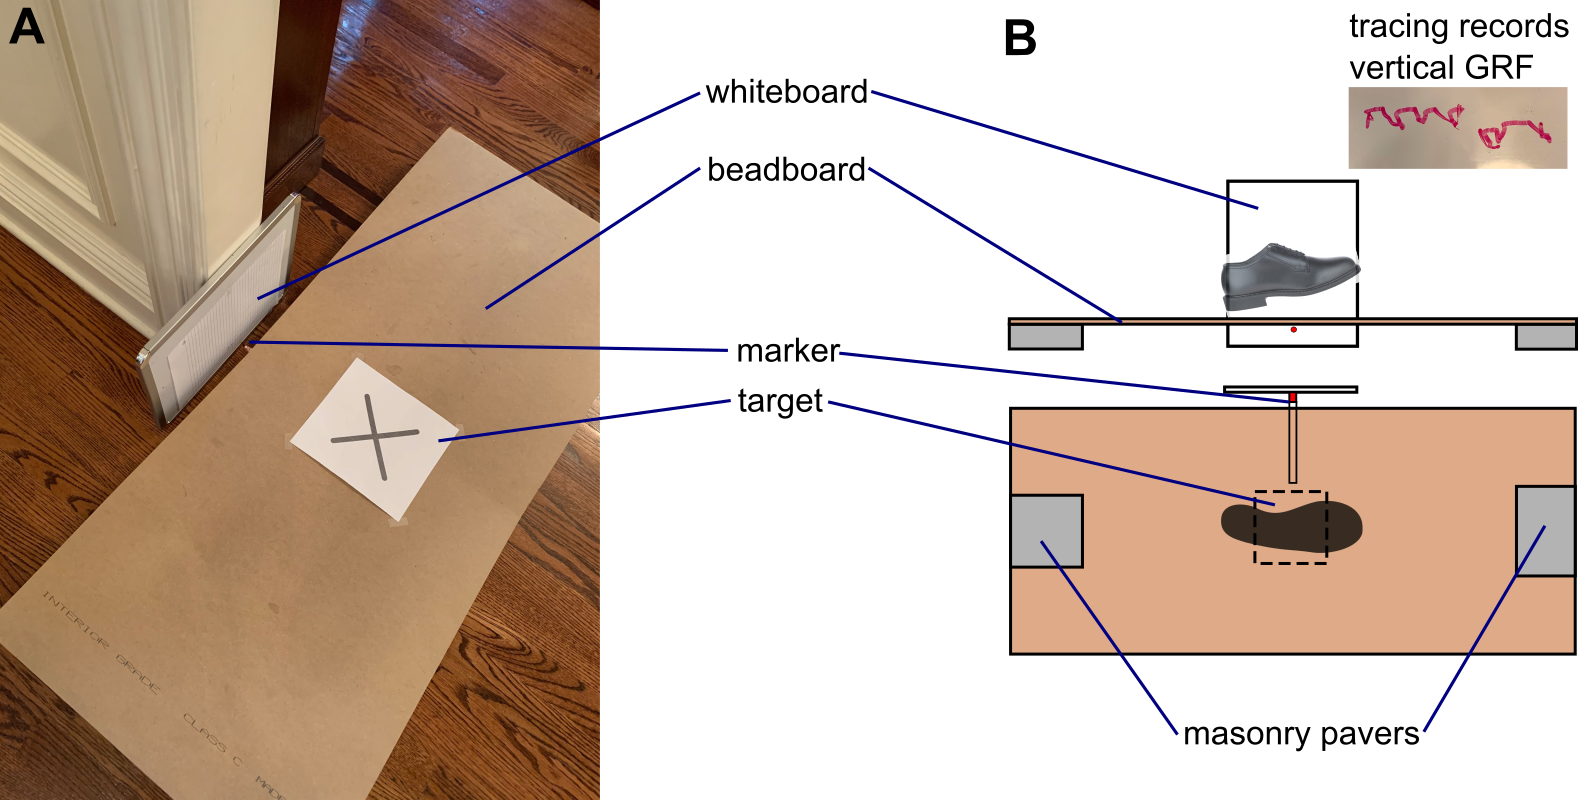
\includegraphics{figures/fig-methods-1.png}
\end{center}
\caption{Improvised one-axis force plate kymograph; (A) complete setup; (B) side and top views and example tracing. As the beadboard flexes under load, the marker traces the lowest point reached, providing a measurement of maximum vertical ground reaction force (GRF). Force plate dimensions \SI{48 x 21 x 0.5}{\inch} (\SI{1.25 x 0.53 x0.013}{\meter}); pavers are \SI{2.25}{\inch} (\SI{0.057}{\meter}) tall.}
\label{fig:methods:forceplate}
\end{figure}
The lowest point reached by the marker is a linear measure of the maximum vertical GRF experienced during contact. Additionally, I found that horizontal GRF would displace the flexure horizontally, providing some indication of their general magnitude. For a point load applied in the middle, the displacement $\delta$ (i.e. marker movement) from point load $F$ (i.e. vertical GRF) is given by \cite{craig2011mechanics}: 
\begin{equation}
\delta = \frac{FL^3}{48 EI},
\label{eq:sensor-response}
\end{equation}
where $E$ is Young's modulus of elasticity, $L$ is the length of the beam, and $I=\frac{1}{12}bh^3$ is the second moment of area; though in practice I simply compared the maximum marker motion rather than perform a detailed calibration of this improvised rig. 

An initial test of the rig failed due to the grooves in the bead board being loaded in tension; the board was replaced with the grooves facing up and was retested first by walking over it. I then took two trials consisting of five steps of heel-strike followed by five steps of forefoot-strike. The white board was moved left approximately \SI{1}{\centi\meter} between steps and \SI{5}{\centi\meter} between treatments to provide visible separation. After each trial, the resulting marker pattern on the white board was photographed using a smartphone camera (iPhone 11; Apple; Cupertino, CA) to allow rough comparison of the magnitude of vertical GRF. forefoot-strike steps appeared to shift the rig laterally; to examine this further I took a third trial consisting of four steps using forefoot-strike, alternating left and right feet. 




\subsection{Measurement of accelerations using a smart phone}
In addition to the rough indication of vertical GRF from the improvised force plate, I measured accelerations in three axes using a smartphone (iPhone 5s; Apple; Cupertino, CA), centered \SI{10}{\centi\meter} below the navel and held in place with the right hand. The method is similar to \citet{shiang2016determine}, who used a multiaxis IMU worn in the shoe; however, that equipment was not available to me. I used the \Matlab\ Mobile app (Mathworks; Natick, MA) to log $X$, $Y$, and $Z$ acceleration at a sampling rate of \SI{100}{\hertz}.  Running was conducted moving straight and level on an empty street about two blocks in length. I recorded \SI{45}{\second} samples of steady running using each running style, at a cadence of approximately \SI{150}{steps\per\minute}, timed using the Avril Lavigne song ``Sk8er Boi''. To avoid end effects during start and stop, I used the middle \SI{10}{\second} segment of each recording for analyses of the acceleration of the center of mass. Analysis of the vertical ($Y$) acceleration measurements was carried out in \Matlab\ (Mathworks; Natick, MA) and R \citep{r2020}, including the \lstinline{tidyverse} and \lstinline{ggplot2} libraries \citep{wickham2019tidyverse}. 



\subsection{Video kinematics on a treadmill}
% In this section or in intro add citations to baker2007history, mayer2010physiological, marey1873locomotion, marey1885method, muybridge1925animals, muybridge1955human, carlet1872essai... 
To examine changes in kinematics and gait during the different running styles, I filmed the subject running on a treadmill (Performance 800; TRUE Fitness; St Louis, MO). Ideally I would have used a high speed camera (TS5; Fastec; San Diego, CA), however, COVID-19 required me to improvise. Instead, I used a smartphone camera (iPhone 11; Apple; Cupertino, CA) filming from the left at approximately \SIrange{1}{2}{\meter}. The camera was held by hand and operated at \SI{30}{\frame\per\second} and \num{1920x1080} pixel resolution. The treadmill was operated at \SI{8}{mph} (\SI{3.6}{\meter\per\second}) for both tests; the subject began running on the treadmill and reached a steady pace before filming.  Two segments were obtained for analysis, \SI{11}{\second} and \SI{13}{\second} in length, for heel-strike and forefoot-strike styles, providing \SI{358}{\frame} and \SI{416}{\frame}, respectively.
\begin{figure}
\begin{center}
\includegraphics{figures/fig-methods-2.png}
\end{center}
\caption{Experimental setup for video kinematics; (A) digitization points at left toe, heel, ankle, knee, hip, and right toe; (B) angle definitions for foot angle ($\alpha$), knee angle ($\beta$) and hip angle ($\gamma$); example manual digitization for (C) heel-strike and (D) forefoot-strike using \lstinline{DLTdv8} \citep{hedrick2008software}.}
\label{fig:methods:kinematics}
\end{figure}

Kinematic analysis proceeded using \citet{hedrick2008software} \lstinline{DLTdv8} (\url{http://biomech.web.unc.edu/dltdv/}) to manually digitize six points (\fref{fig:methods:kinematics}) in each frame of video: (1) left toe at the front of the white sole; (2) left heel at the back of the white sole; (3) left ankle at the lateral malleolus as judged by white ankle socks worn by the subject; (4) left knee as judged by the bump from the lateral condyles of the femur and tibia; (5) left hip as judged from a faint stripe marking on the subject's athletic shorts. In addition, a sixth point, the right toe, was also digitized in order to confirm that the left-right phase was \ang{90}. 

Specially written code in \Matlab\ was used to convert the digitized point locations into the joint angles depicted in \fref{fig:methods:kinematics}. The joint angle definitions followed those used in previous human locomotion studies \citep{qiao2016leg, giandolini2013impact, larson2014comparison, hamner2010muscle, liu2008muscle, dickinson1985measurement, mcmahon1984muscles}. Foot angle ($\alpha$) was defined with \ang{0} as anatomically neutral position, positive $\alpha$ as dorsiflexion, and negative $\alpha$ as plantar flexion. The knee angle ($\beta$) was defined with \ang{0} as anatomically neutral position, and positive $\beta$ as knee flexion. Hip angle ($\gamma$) was defined with \ang{0} as anatomically neutral position, positive $\gamma$ as flexion, and negative $\gamma$ as extension. As a sanity check, the joint angles I observed were similar to those in high speed walking \citep{liu2008muscle}. I attempted to fit these to a periodic function using Fourier series but found a large number of terms was needed and that the fits achieved were mediocre; a means of decomposing a piecewise continuous time series for joint angles (due to the non-smooth nature of intermittent contact, stance and swing in bipedal and polypedal locomotion) is needed. 

In addition to joint angle, phase was recovered using a method based on the Phaser algorithm \citep{revzen2008estimating}, by taking the principal component analysis (PCA) of all the six digitized points' $x$ and $y$ coordinates, then finding the phase angle of the Hilbert transform of the first principal component (PC1). The phase was then adjusted to range from 0 to $2\pi$ \citep{revzen2009towards}, with 0 phase corresponding to the beginning of the first recorded stance phase. This allows comparison of each of the 17 and 21 steps in the heel-strike and forefoot-strike analysis videos, respectively. Phase calculations were carried out in \Matlab\ and made use of the \lstinline{pca} and \lstinline{hilbert} functions. 
% can we get how much of variance covered in PC1,2 components? 

To allow for comparison of stride frequency, stride period, and duty cycle, the videos were reviewed frame by frame in \lstinline{DLTdv8} to identify (1) the start of stance phase based on toe or heel contact; (2) end of stance phase judged by toe liftoff; and (3) toe contact (for heel-strike trials) to aid in length and speed calibration.  For heel-strike analysis, start of stance was judged by heel-strike and rapid foot plantar flexion in contact with the ground; for forefoot-strike analysis, start of stance was judged by observing when the toe struck the ground during plantar flexion. The angle from the point of contact (heel or toe) to the hip, and the angle of the ankle were also computed as part of this analysis. Additional plotting and statistical analyses were completed in \Matlab\ and R \citep{r2020}. 

\begin{figure}
\begin{center}
%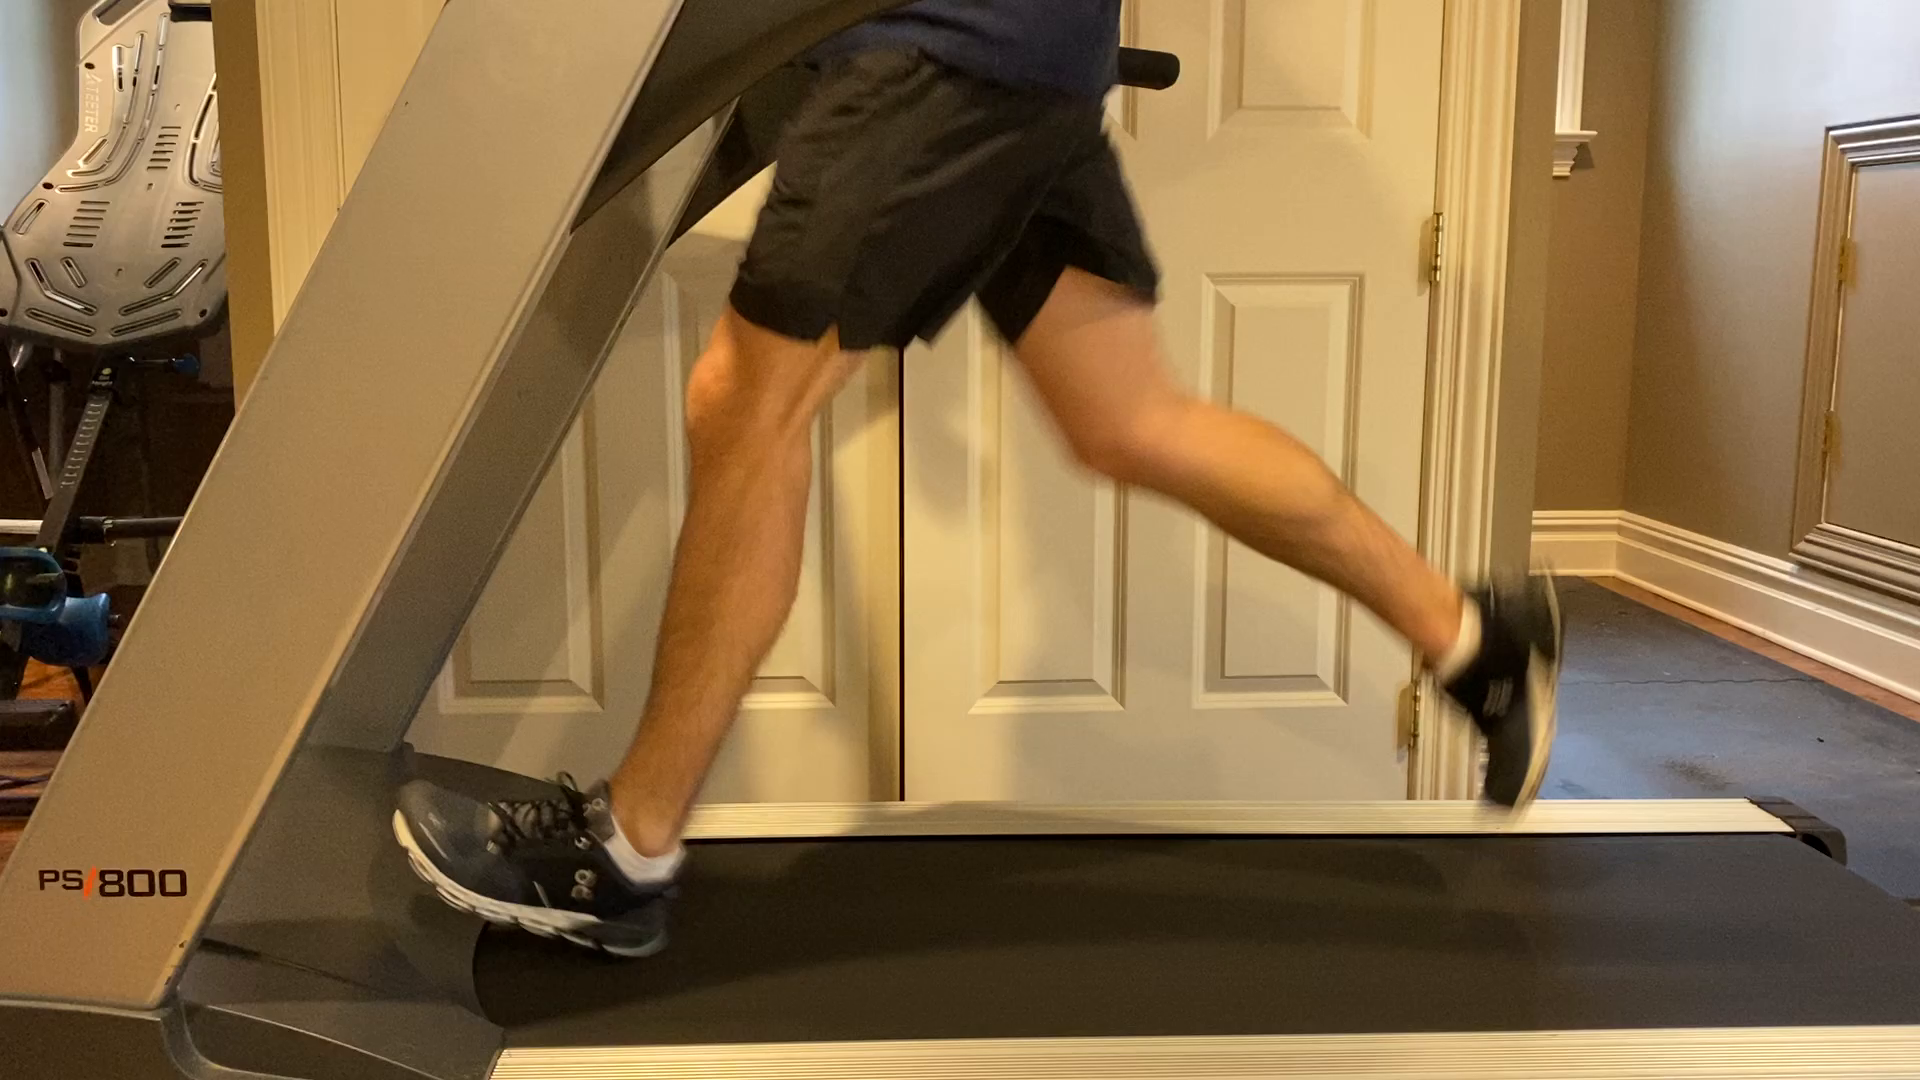
\includegraphics[width=0.29\columnwidth]{figures/heel_frames1.png}
%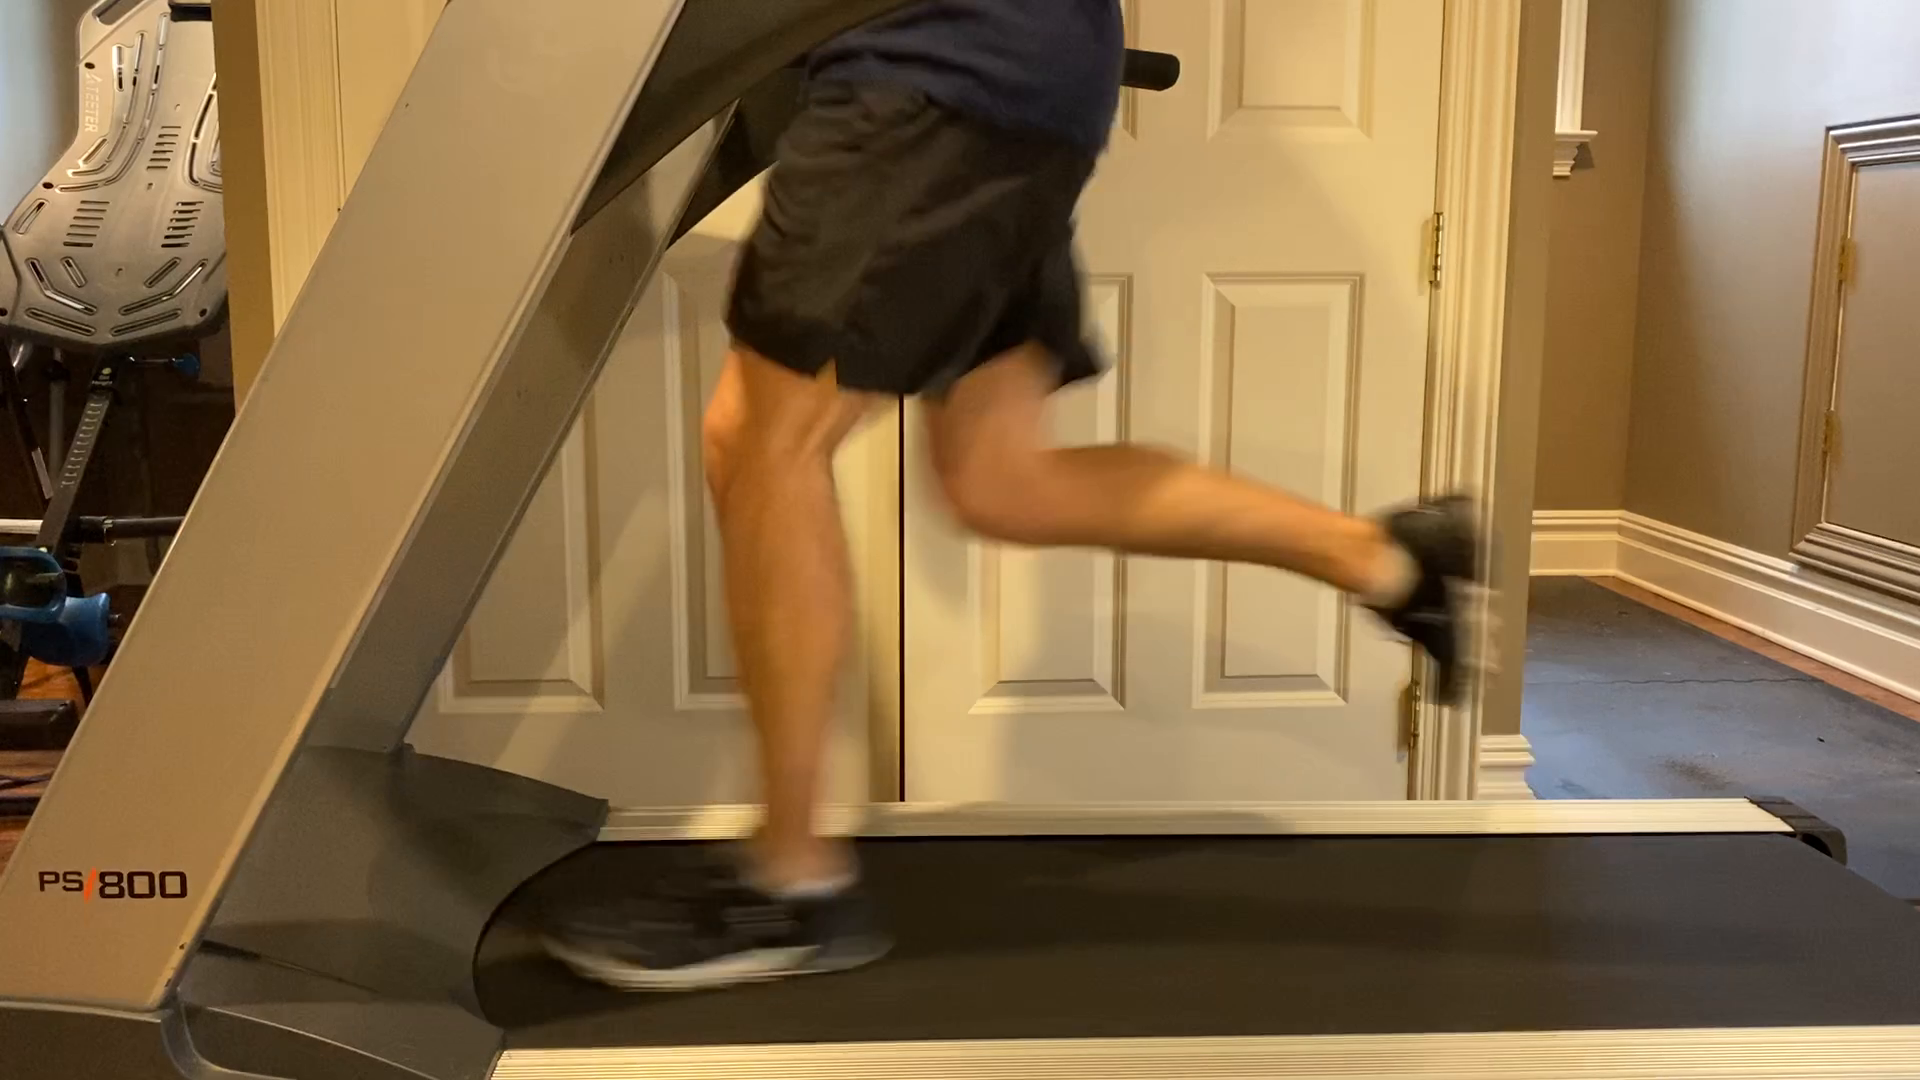
\includegraphics[width=0.29\columnwidth]{figures/heel_frames3.png}
%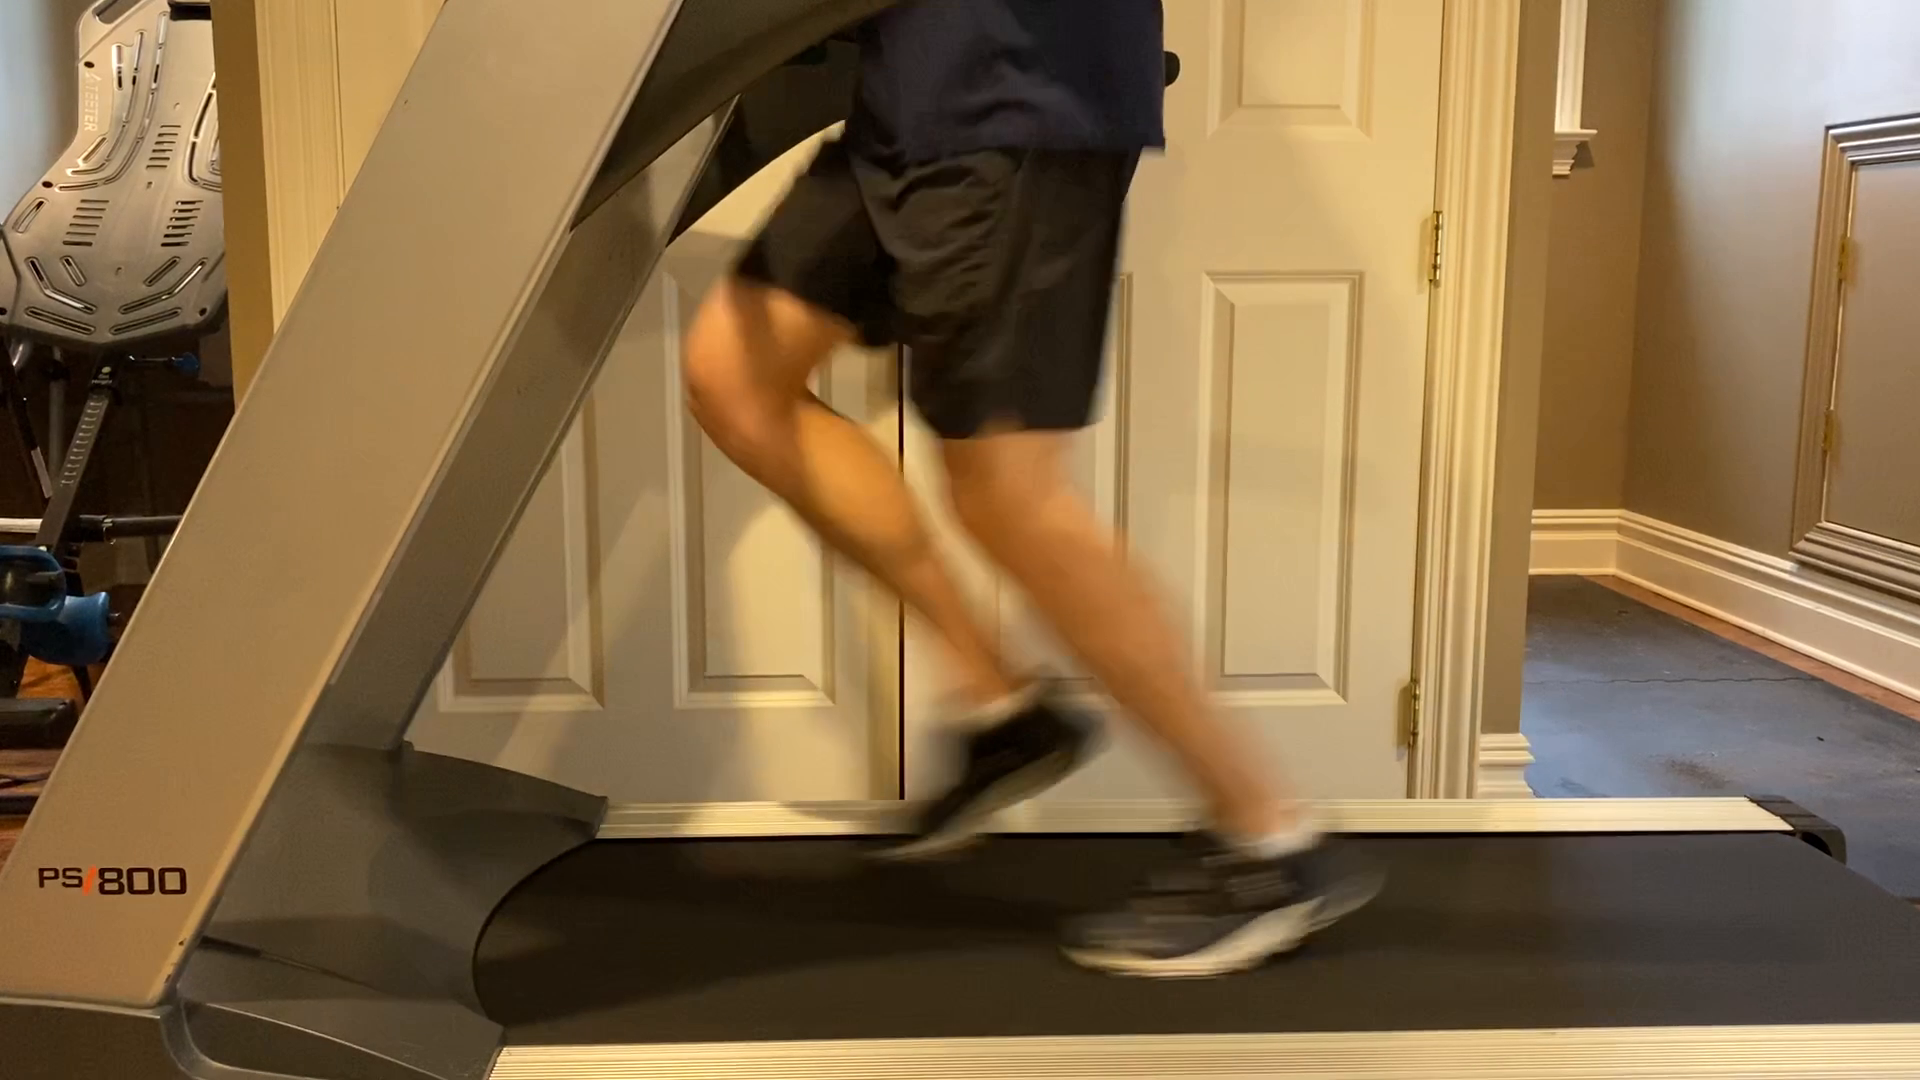
\includegraphics[width=0.29\columnwidth]{figures/heel_frames7.png}\\
%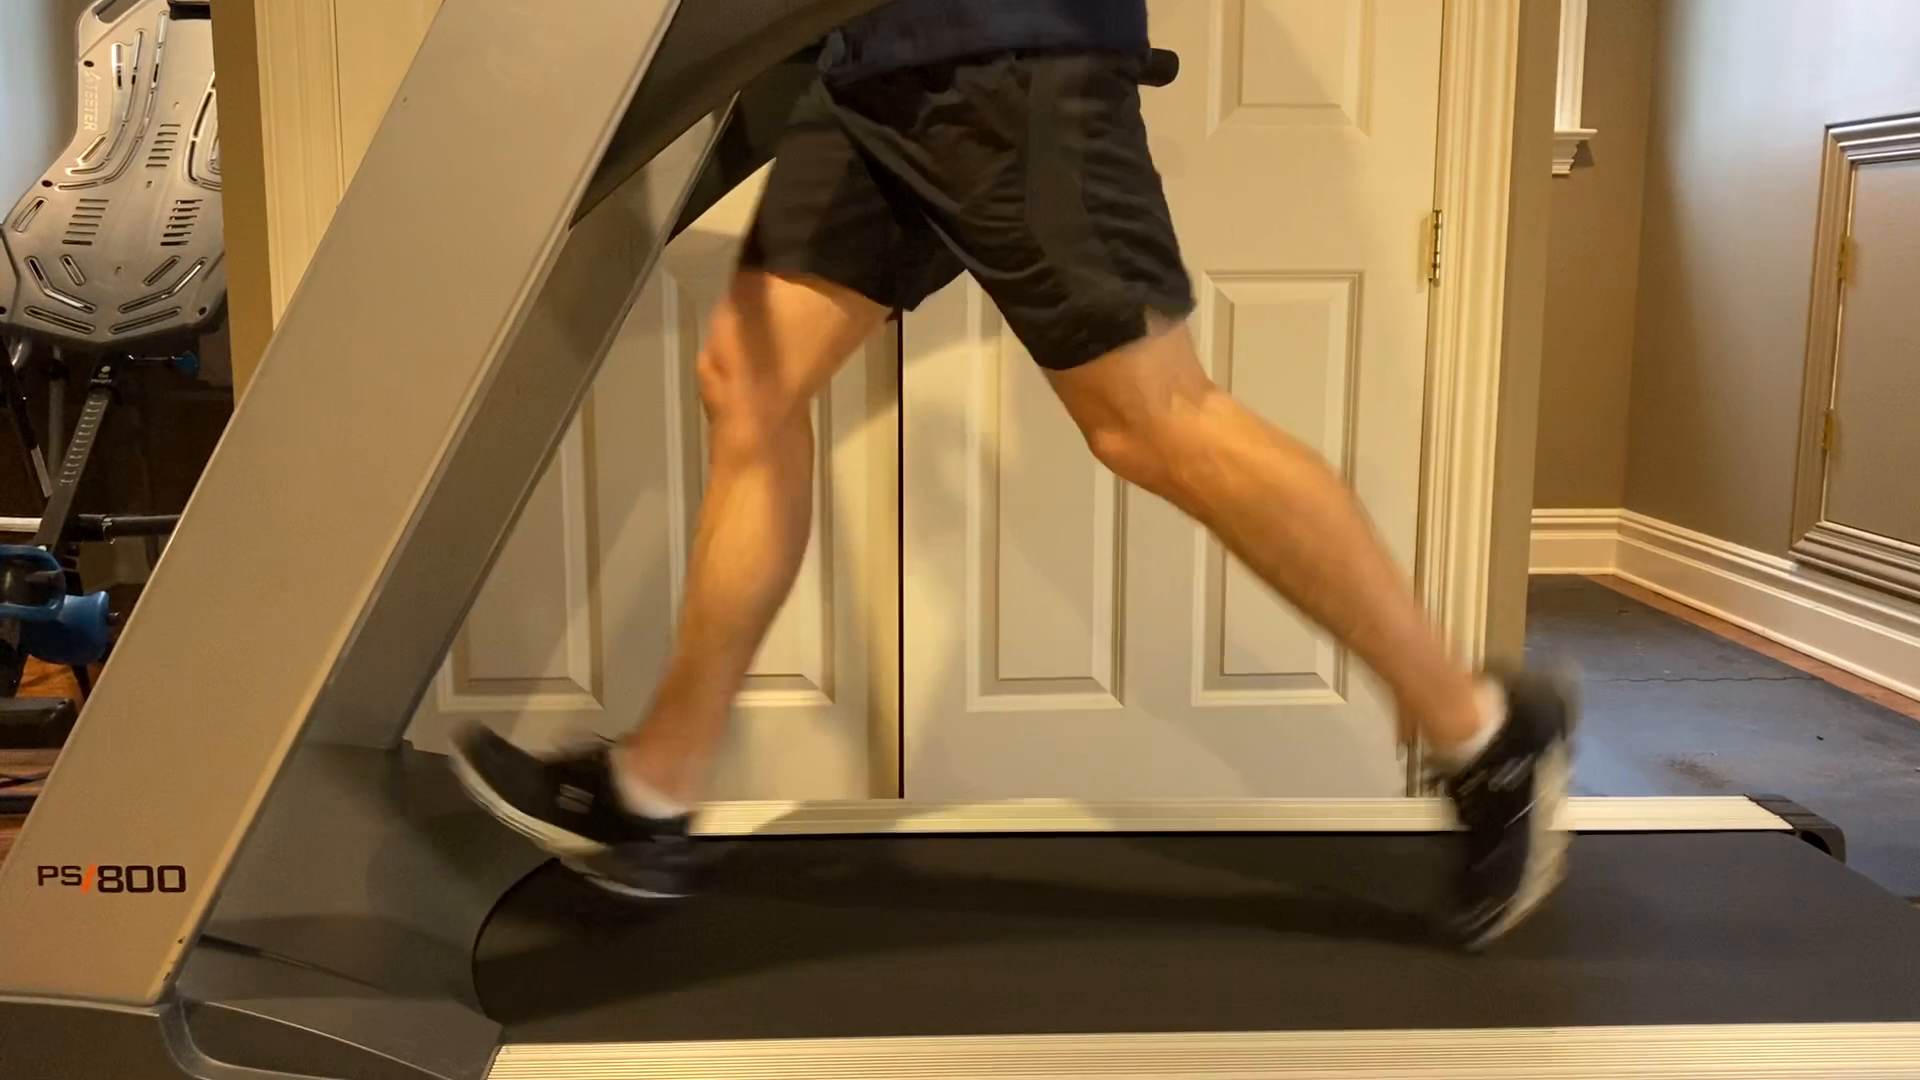
\includegraphics[width=0.29\columnwidth]{figures/heel_frames10.png}
%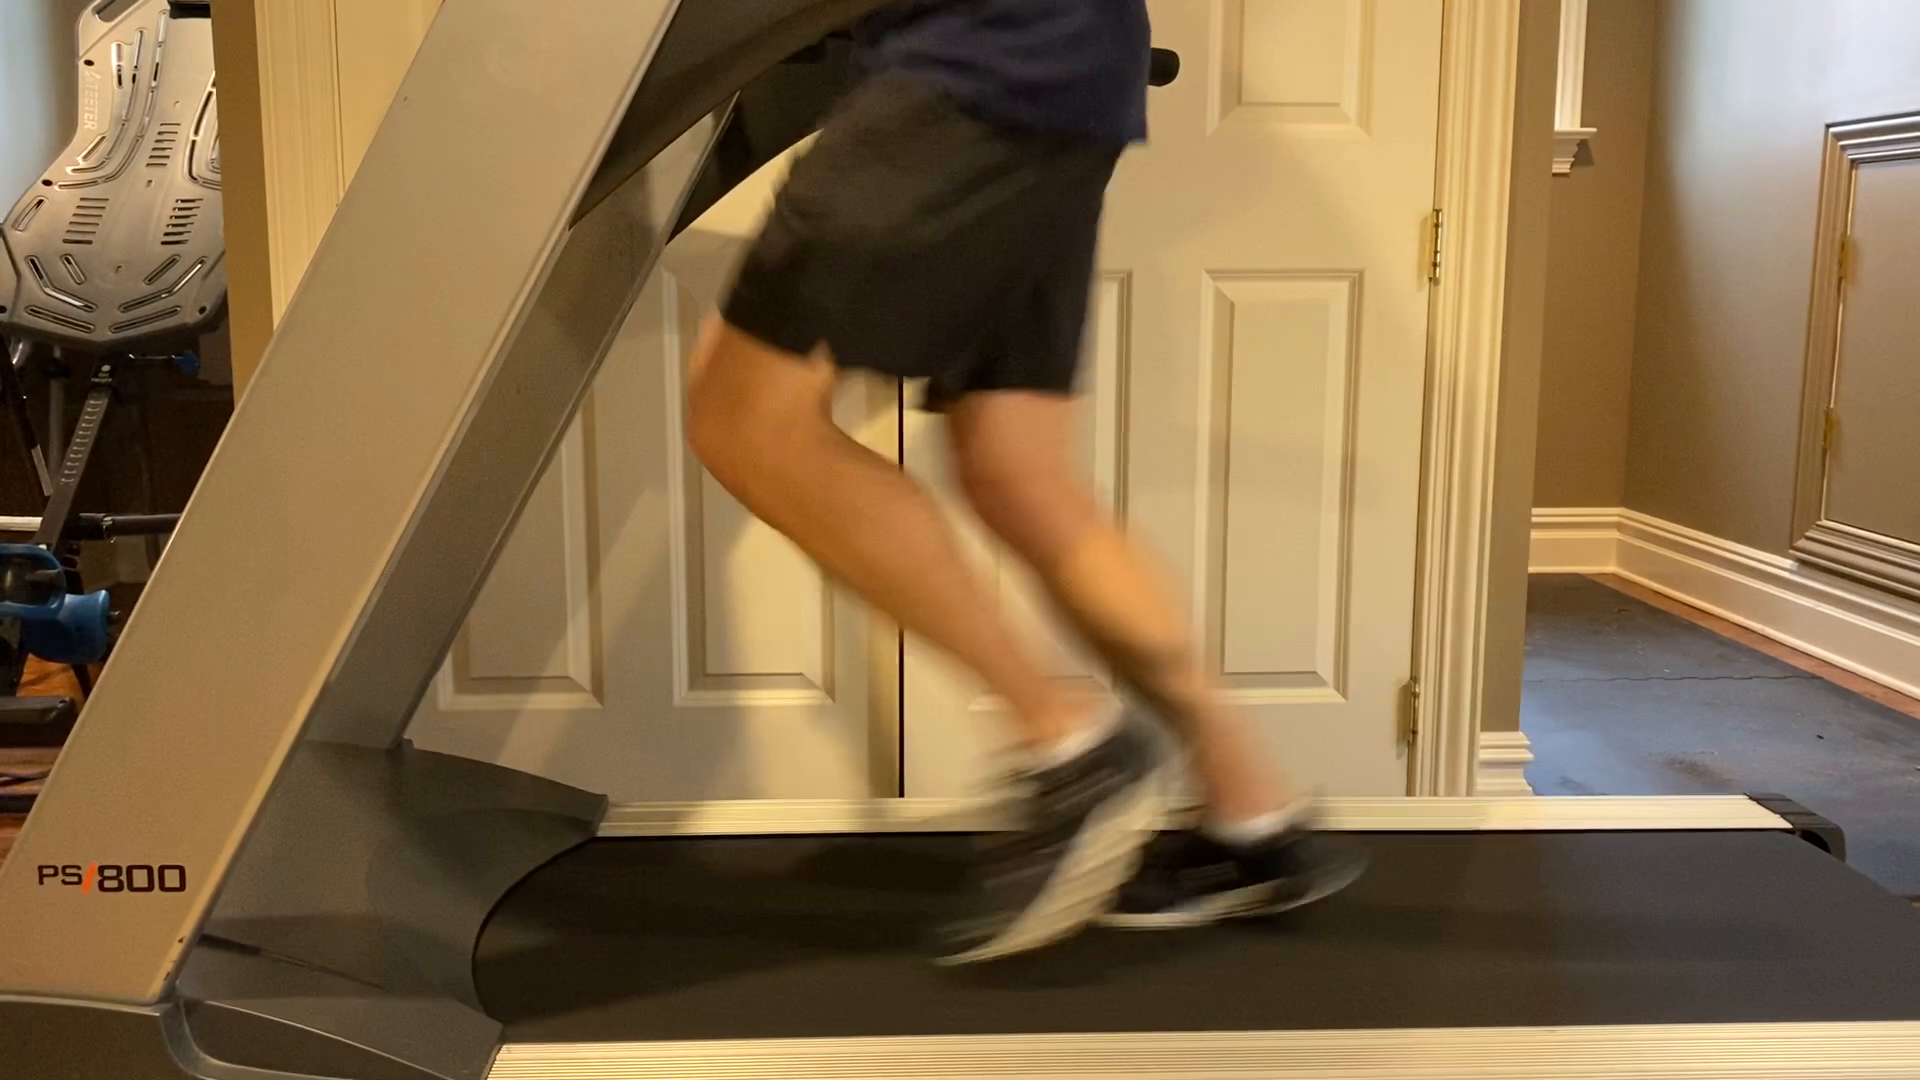
\includegraphics[width=0.29\columnwidth]{figures/heel_frames17.png}
%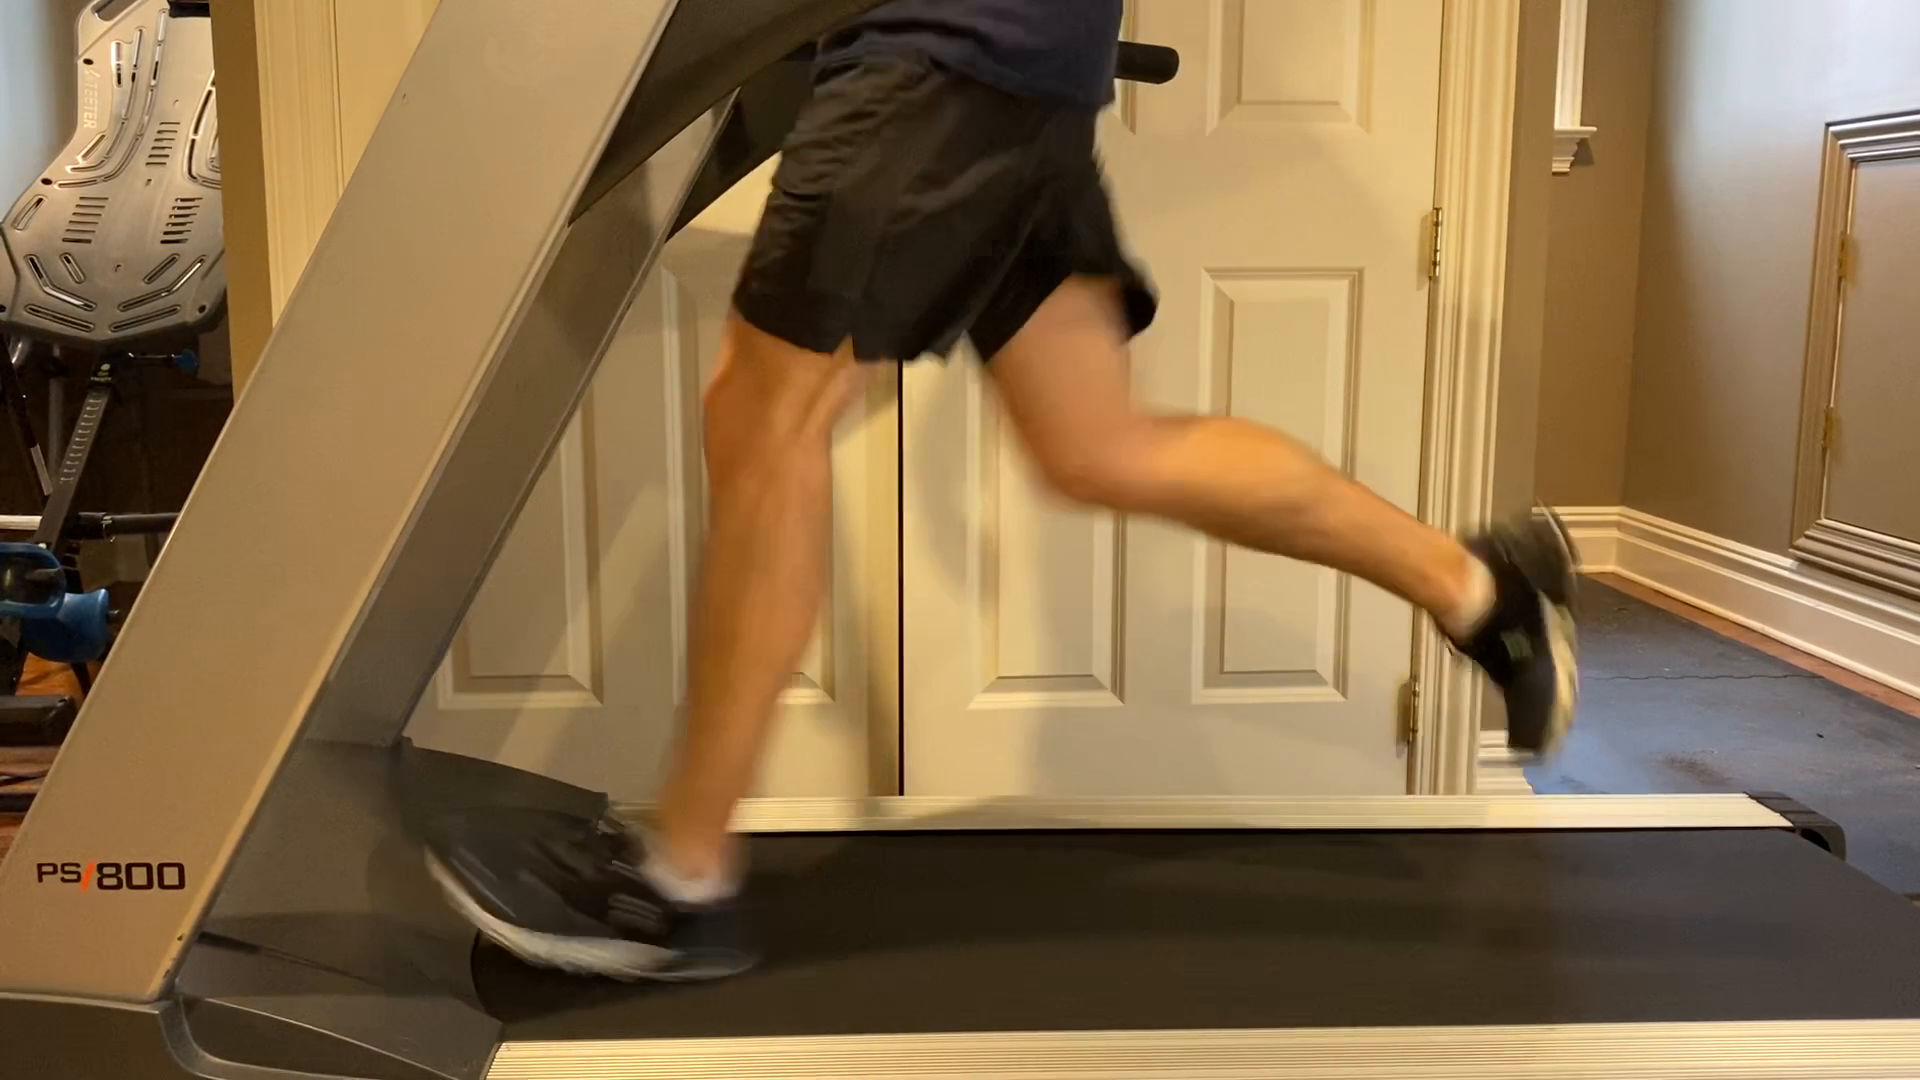
\includegraphics[width=0.29\columnwidth]{figures/heel_frames22.png}
\includegraphics{figures/fig-methods-3.png}
\end{center}
\caption{Example video frames from running on a treadmill at \SI{8}{mph} (\SI{3.6}{\meter\per\second}), showing (A) heel-strike; (B) toe down; (C) intermediate during stance; (D) toe up; (E) intermediate during swing; and (F) start of the next step. Frame times marked.} 
\label{fig:methods:dltdv8-2}
\end{figure}


